\chapter{Pretraining Engineering}

Pretraining is the process of teaching a base language model from raw text. The mathematical objective is simple: predict the next token. The engineering system around that objective is where many real projects succeed or fail.

At undergraduate scale, pretraining might mean a tiny corpus, a tiny model, and one CPU or GPU. At professional scale, it may mean trillions of tokens, many machines, distributed checkpointing, and careful monitoring. The logic is the same. The difference is scale, cost, and discipline.

\section{Chapter Goals}

By the end of this chapter, you should be able to:

\begin{itemize}
  \item describe the full pretraining system around TinyGPT;
  \item explain how raw documents become token shards and then batches;
  \item design a reproducible run directory with configs, logs, and checkpoints;
  \item state what a checkpoint must contain for faithful resume;
  \item explain validation, checkpoint cadence, and sample monitoring;
  \item compute effective batch size and tokens processed;
  \item understand the basic shape of distributed data parallel training;
  \item diagnose common pretraining failures with a practical runbook.
\end{itemize}

\section{Pretraining Is A System, Not Just A Loop}

The training loop is the center, but it depends on many surrounding artifacts:

\begin{center}
\resizebox{\textwidth}{!}{
\begin{tikzpicture}[
  box/.style={draw, rounded corners=2pt, minimum height=0.66cm, text width=2.25cm, align=center},
  arrow/.style={-{Latex[length=2mm]}, thick},
  note/.style={font=\small, align=center}
]
\node[box, fill=blue!5] (docs) at (0,0) {raw documents};
\node[box, fill=blue!5] (clean) at (2.8,0) {clean/filter};
\node[box, fill=yellow!18] (tok) at (5.6,0) {tokenizer};
\node[box, fill=yellow!18] (shards) at (8.4,0) {token shards\\\texttt{.bin}};
\node[box, fill=red!8] (loader) at (11.2,0) {data loader};
\node[box, fill=red!8] (train) at (14.0,0) {training loop};
\node[box, fill=green!10] (ckpt) at (14.0,-1.2) {checkpoints};
\node[box, fill=green!10] (logs) at (11.2,-1.2) {logs + metrics};
\node[box, fill=green!10] (val) at (8.4,-1.2) {validation};
\draw[arrow] (docs) -- (clean);
\draw[arrow] (clean) -- (tok);
\draw[arrow] (tok) -- (shards);
\draw[arrow] (shards) -- (loader);
\draw[arrow] (loader) -- (train);
\draw[arrow] (train) -- (ckpt);
\draw[arrow] (train) -- (logs);
\draw[arrow] (train) -- (val);
\node[note] at (7.0,-2.1) {Pretraining quality depends on data, config, code, checkpoints, and monitoring together.};
\end{tikzpicture}}
\end{center}

When a run fails, the bug may be in the model, but it may also be in tokenization, target shifting, shard boundaries, config, device placement, optimizer state, or validation split.

\section{The Pretraining Loop}

A minimal pretraining loop is:

\begin{lstlisting}
load config
load tokenizer metadata
load token dataset
initialize model
initialize optimizer
repeat:
    sample a batch
    run forward pass
    compute loss
    run backward pass
    update parameters
    log metrics
    periodically validate
    periodically save checkpoint
\end{lstlisting}

In code, the loop is short. In engineering, each line is a contract.

\begin{center}
\begin{tikzpicture}[
  box/.style={draw, rounded corners=2pt, minimum height=0.62cm, text width=2.15cm, align=center},
  arrow/.style={-{Latex[length=2mm]}, thick}
]
\node[box, fill=blue!5] (cfg) at (0,1.2) {config};
\node[box, fill=blue!5] (data) at (0,0) {token data};
\node[box, fill=blue!5] (seed) at (0,-1.2) {seed};
\node[box, fill=red!8] (loop) at (3.6,0) {training loop};
\node[box, fill=green!10] (metrics) at (7.0,1.2) {metrics};
\node[box, fill=green!10] (ckpt) at (7.0,0) {checkpoint};
\node[box, fill=green!10] (samples) at (7.0,-1.2) {samples};
\draw[arrow] (cfg) -- (loop);
\draw[arrow] (data) -- (loop);
\draw[arrow] (seed) -- (loop);
\draw[arrow] (loop) -- (metrics);
\draw[arrow] (loop) -- (ckpt);
\draw[arrow] (loop) -- (samples);
\end{tikzpicture}
\end{center}

Good pretraining is not merely running the loop. It is making the loop explainable after it finishes.

\section{From Documents To Token Shards}

Training does not usually read raw text directly. It reads token IDs. The pipeline is:

\[
\text{documents}\rightarrow\text{normalized text}\rightarrow\text{token IDs}\rightarrow\text{binary shards}.
\]

\begin{center}
\resizebox{0.96\textwidth}{!}{
\begin{tikzpicture}[
  box/.style={draw, rounded corners=2pt, minimum height=0.66cm, text width=2.25cm, align=center},
  arrow/.style={-{Latex[length=2mm]}, thick},
  note/.style={font=\small, align=center}
]
\node[box, fill=blue!5] (doc1) at (0,0.8) {doc 1\\text};
\node[box, fill=blue!5] (doc2) at (0,-0.1) {doc 2\\text};
\node[box, fill=blue!5] (doc3) at (0,-1.0) {doc 3\\text};
\node[box, fill=yellow!18] (clean) at (3,0) {clean +\\deduplicate};
\node[box, fill=yellow!18] (encode) at (6,0) {encode\\token IDs};
\node[box, fill=red!8] (stream) at (9,0) {token stream\\\([2,3,4,\ldots]\)};
\node[box, fill=green!10] (shards) at (12,0) {shards\\{\footnotesize\texttt{train\_000.bin}}};
\draw[arrow] (doc1) -- (clean);
\draw[arrow] (doc2) -- (clean);
\draw[arrow] (doc3) -- (clean);
\draw[arrow] (clean) -- (encode);
\draw[arrow] (encode) -- (stream);
\draw[arrow] (stream) -- (shards);
\node[note] at (6,-1.45) {The model only sees token IDs; data quality decisions happen before training.};
\end{tikzpicture}}
\end{center}

For the \texttt{llm-train} project, a token shard should have explicit metadata:

\begin{lstlisting}
data/tokens/tinygpt/
  train_000.bin
  train_001.bin
  val_000.bin
  metadata.json
\end{lstlisting}

The metadata should record:

\begin{itemize}
  \item tokenizer name and vocabulary size;
  \item dtype, such as \texttt{uint16} or \texttt{uint32};
  \item byte order, preferably little-endian;
  \item number of tokens per shard;
  \item source corpus and license notes;
  \item preprocessing version and date;
  \item checksum for each shard.
\end{itemize}

\section{Binary Token Format}

Text is expensive to parse repeatedly. A binary token file is a contiguous array of token IDs:

\[
\texttt{train.bin} =
\begin{bmatrix}
2&3&4&5&6&7&8&\cdots
\end{bmatrix}.
\]

\begin{center}
\resizebox{0.95\textwidth}{!}{
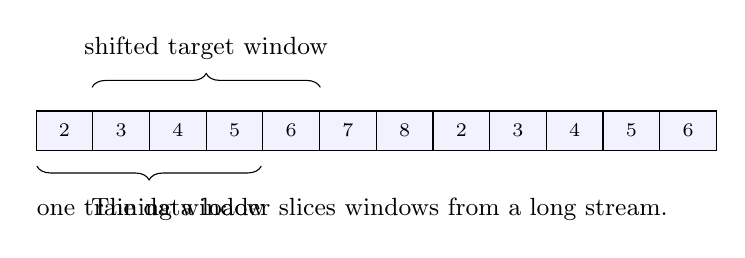
\begin{tikzpicture}[
  cell/.style={draw, minimum width=0.72cm, minimum height=0.5cm, align=center},
  note/.style={font=\small, align=center},
  arrow/.style={-{Latex[length=2mm]}, thick}
]
\foreach \i/\v in {0/2,1/3,2/4,3/5,4/6,5/7,6/8,7/2,8/3,9/4,10/5,11/6} {
  \node[cell, fill=blue!5] (c\i) at (\i*0.72,0) {\scriptsize \v};
}
\draw[decorate, decoration={brace, mirror, amplitude=5pt}] (-0.35,-0.45) -- (2.5,-0.45);
\node[note] at (1.1,-1.0) {one training window};
\draw[decorate, decoration={brace, amplitude=5pt}] (0.35,0.55) -- (3.25,0.55);
\node[note] at (1.8,1.05) {shifted target window};
\node[note] at (4.0,-1.0) {The data loader slices windows from a long stream.};
\end{tikzpicture}}
\end{center}

For context length \(T\), a sample starting at index \(s\) is:

\[
x = \texttt{tokens}[s:s+T],
\]

\[
y = \texttt{tokens}[s+1:s+T+1].
\]

This one-token shift is the training target alignment.

\section{Batch Sampling}

A batch contains many windows:

\[
x\in\mathbb{Z}^{B\times T},
\qquad
y\in\mathbb{Z}^{B\times T}.
\]

\begin{center}
\resizebox{0.85\textwidth}{!}{
\begin{tikzpicture}[
  cell/.style={draw, minimum width=0.62cm, minimum height=0.46cm, align=center},
  note/.style={font=\small, align=center},
  arrow/.style={-{Latex[length=2mm]}, thick}
]
\node[note] at (1.25,0.75) {input batch \(x\)};
\foreach \r in {0,1,2} {
  \foreach \c in {0,1,2,3,4} {
    \node[cell, fill=blue!5] at (\c*0.62,-\r*0.48) {};
  }
}
\node[note] at (5.2,0.75) {target batch \(y\)};
\foreach \r in {0,1,2} {
  \foreach \c in {0,1,2,3,4} {
    \node[cell, fill=red!8] at (4.0+\c*0.62,-\r*0.48) {};
  }
}
\draw[arrow] (3.05,-0.48) -- (3.75,-0.48);
\node[note] at (3.5,-2.1) {Every row in \(y\) is the corresponding row in \(x\), shifted by one token.};
\end{tikzpicture}}
\end{center}

Minimal data loader logic:

\begin{lstlisting}[language=Python]
def get_batch(split):
    data = train_data if split == "train" else val_data
    ix = torch.randint(0, len(data) - block_size - 1, (batch_size,))
    x = torch.stack([data[i:i+block_size] for i in ix])
    y = torch.stack([data[i+1:i+block_size+1] for i in ix])
    return x.to(device), y.to(device)
\end{lstlisting}

Professional loaders avoid Python loops and use memory mapping or streaming, but the contract is the same.

\section{Configuration Discipline}

Training should be driven by explicit config files. A config records:

\begin{itemize}
  \item model size;
  \item tokenizer and dataset paths;
  \item batch size, block size, and gradient accumulation;
  \item optimizer hyperparameters;
  \item learning-rate schedule;
  \item validation interval;
  \item checkpoint interval;
  \item random seed;
  \item hardware assumptions.
\end{itemize}

\begin{center}
\begin{tikzpicture}[
  box/.style={draw, rounded corners=2pt, minimum height=0.62cm, text width=2.45cm, align=center},
  arrow/.style={-{Latex[length=2mm]}, thick}
]
\node[box, fill=blue!5] (cfg) at (0,0) {\texttt{tiny.yaml}};
\node[box, fill=red!8] (model) at (3.2,1.0) {model\\shape};
\node[box, fill=yellow!18] (data) at (3.2,0) {data\\paths};
\node[box, fill=green!10] (optim) at (3.2,-1.0) {optimizer\\schedule};
\node[box, fill=gray!12] (run) at (6.4,0) {run directory};
\draw[arrow] (cfg) -- (model);
\draw[arrow] (cfg) -- (data);
\draw[arrow] (cfg) -- (optim);
\draw[arrow] (model) -- (run);
\draw[arrow] (data) -- (run);
\draw[arrow] (optim) -- (run);
\end{tikzpicture}
\end{center}

Do not rely on memory or shell history to explain a run. A future student should be able to read a config and understand exactly what was attempted.

\section{Run Directories}

Every serious run should write to a run directory:

\begin{lstlisting}
runs/
  2026-05-12-tinygpt-smoke/
    config.yaml
    resolved_config.json
    tokenizer.json
    dataset_card.md
    metrics.jsonl
    samples/
      step_000000.txt
      step_001000.txt
    checkpoints/
      step_000000.pt
      step_001000.pt
      latest.pt
    logs/
      train.log
\end{lstlisting}

\begin{center}
\resizebox{0.9\textwidth}{!}{
\begin{tikzpicture}[
  box/.style={draw, rounded corners=2pt, minimum height=0.62cm, text width=2.35cm, align=center},
  arrow/.style={-{Latex[length=2mm]}, thick},
  note/.style={font=\small, align=center}
]
\node[box, fill=blue!5] (run) at (0,0) {run directory};
\node[box, fill=yellow!18] (cfg) at (3,1.2) {configs +\\metadata};
\node[box, fill=red!8] (metrics) at (3,0.4) {metrics\\JSONL};
\node[box, fill=green!10] (ckpts) at (3,-0.4) {checkpoints};
\node[box, fill=gray!12] (samples) at (3,-1.2) {samples};
\draw[arrow] (run) -- (cfg);
\draw[arrow] (run) -- (metrics);
\draw[arrow] (run) -- (ckpts);
\draw[arrow] (run) -- (samples);
\node[note] at (3,-2.0) {A run directory is a scientific record of an experiment.};
\end{tikzpicture}}
\end{center}

This structure also makes it easier to later build dashboards, course labs, or MapleAI learning pages from training runs.

\section{Reproducibility}

Reproducibility means another run can reasonably recreate the result. Perfect determinism is difficult on GPUs, but disciplined metadata is still essential.

Record:

\begin{lstlisting}
git commit
dirty working tree status
config file
resolved config
tokenizer metadata
dataset checksum
software versions
hardware summary
random seed
checkpoint step
\end{lstlisting}

\begin{center}
\begin{tikzpicture}[
  box/.style={draw, rounded corners=2pt, minimum height=0.62cm, text width=2.35cm, align=center},
  arrow/.style={-{Latex[length=2mm]}, thick}
]
\node[box, fill=blue!5] (code) at (0,1.0) {code\\commit};
\node[box, fill=blue!5] (data) at (0,0) {data\\checksum};
\node[box, fill=blue!5] (cfg) at (0,-1.0) {config\\seed};
\node[box, fill=red!8] (run) at (3.2,0) {training run};
\node[box, fill=green!10] (result) at (6.4,0) {explainable\\result};
\draw[arrow] (code) -- (run);
\draw[arrow] (data) -- (run);
\draw[arrow] (cfg) -- (run);
\draw[arrow] (run) -- (result);
\end{tikzpicture}
\end{center}

If two runs differ, this metadata helps locate why.

\section{Checkpoints}

A useful checkpoint should include:

\begin{itemize}
  \item model parameters;
  \item optimizer state;
  \item scheduler state or current step;
  \item random number generator states when possible;
  \item model config;
  \item tokenizer identity;
  \item dataset identity;
  \item training step and tokens processed.
\end{itemize}

Saving only weights is enough for some inference use cases, but not enough to resume training faithfully.

\begin{center}
\resizebox{0.92\textwidth}{!}{
\begin{tikzpicture}[
  box/.style={draw, rounded corners=2pt, minimum height=0.62cm, text width=2.45cm, align=center},
  arrow/.style={-{Latex[length=2mm]}, thick}
]
\node[box, fill=blue!5] (model) at (0,1.2) {model\\weights};
\node[box, fill=yellow!18] (opt) at (0,0.4) {optimizer\\moments};
\node[box, fill=yellow!18] (sched) at (0,-0.4) {scheduler\\step};
\node[box, fill=red!8] (meta) at (0,-1.2) {config +\\metadata};
\node[box, fill=green!10] (ckpt) at (4,0) {checkpoint};
\node[box, fill=gray!12] (resume) at (8,0) {faithful\\resume};
\draw[arrow] (model) -- (ckpt);
\draw[arrow] (opt) -- (ckpt);
\draw[arrow] (sched) -- (ckpt);
\draw[arrow] (meta) -- (ckpt);
\draw[arrow] (ckpt) -- (resume);
\end{tikzpicture}}
\end{center}

\section{Checkpoint Cadence}

Saving too often wastes time and storage. Saving too rarely risks losing work. A practical policy:

\begin{itemize}
  \item always save an initial checkpoint after model creation;
  \item save \texttt{latest.pt} frequently for recovery;
  \item save numbered checkpoints less frequently for milestones;
  \item save best validation checkpoint separately;
  \item keep a retention policy so disk does not fill.
\end{itemize}

\begin{center}
\resizebox{0.95\textwidth}{!}{
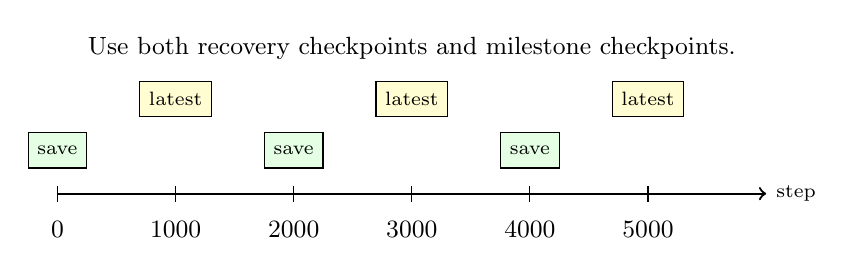
\begin{tikzpicture}[
  tick/.style={draw, minimum width=0.5cm, minimum height=0.45cm, align=center},
  note/.style={font=\small, align=center}
]
\draw[->, thick] (0,0) -- (9,0) node[right] {\scriptsize step};
\foreach \x/\lab in {0/0,1.5/1000,3/2000,4.5/3000,6/4000,7.5/5000} {
  \draw (\x,0.1) -- (\x,-0.1);
  \node[note] at (\x,-0.45) {\lab};
}
\foreach \x in {0,3,6} {
  \node[tick, fill=green!10] at (\x,0.55) {\scriptsize save};
}
\foreach \x in {1.5,4.5,7.5} {
  \node[tick, fill=yellow!18] at (\x,1.2) {\scriptsize latest};
}
\node[note] at (4.5,1.85) {Use both recovery checkpoints and milestone checkpoints.};
\end{tikzpicture}}
\end{center}

\section{Validation}

Validation estimates performance on held-out data. The validation set must not be used for training. The usual validation loss is the same cross-entropy loss, computed with the model in evaluation mode:

\begin{lstlisting}[language=Python]
model.eval()
with torch.no_grad():
    val_loss = estimate_loss("val")
model.train()
\end{lstlisting}

Evaluation mode matters because dropout behaves differently during training and evaluation. \texttt{torch.no\_grad()} matters because validation does not need gradients, so it saves memory.

\begin{center}
\begin{tikzpicture}[
  box/.style={draw, rounded corners=2pt, minimum height=0.62cm, text width=2.4cm, align=center},
  arrow/.style={-{Latex[length=2mm]}, thick}
]
\node[box, fill=blue!5] (train) at (0,0.7) {train split\\updates model};
\node[box, fill=green!10] (val) at (0,-0.7) {validation split\\measures model};
\node[box, fill=red!8] (model) at (3.6,0.7) {forward +\\backward};
\node[box, fill=yellow!18] (eval) at (3.6,-0.7) {forward only\\no gradients};
\node[box, fill=gray!12] (logs) at (7.0,0) {loss curves};
\draw[arrow] (train) -- (model);
\draw[arrow] (val) -- (eval);
\draw[arrow] (model) -- (logs);
\draw[arrow] (eval) -- (logs);
\end{tikzpicture}
\end{center}

\section{Sampling During Training}

Validation loss is useful, but samples are also important. A sample is not a scientific metric by itself, but it reveals obvious failures:

\begin{itemize}
  \item tokenizer mismatch;
  \item repeated punctuation;
  \item endless loops;
  \item broken decoding;
  \item checkpoint loading mistakes.
\end{itemize}

Sampling should use a fixed prompt at fixed intervals so progress can be compared:

\begin{lstlisting}
Prompt: "Tiny GPT"
step 0:      random-looking tokens
step 1000:   more local structure
step 5000:   memorized tiny corpus or plausible continuation
\end{lstlisting}

\begin{center}
\begin{tikzpicture}[
  box/.style={draw, rounded corners=2pt, minimum height=0.62cm, text width=2.35cm, align=center},
  arrow/.style={-{Latex[length=2mm]}, thick}
]
\node[box, fill=blue!5] (prompt) at (0,0) {fixed prompt};
\node[box, fill=red!8] (model) at (3,0) {checkpointed\\model};
\node[box, fill=green!10] (sample) at (6,0) {sample text};
\node[box, fill=yellow!18] (compare) at (9,0) {compare\\over steps};
\draw[arrow] (prompt) -- (model);
\draw[arrow] (model) -- (sample);
\draw[arrow] (sample) -- (compare);
\end{tikzpicture}
\end{center}

\section{Tokens Processed And Effective Batch Size}

Training progress is often measured in tokens:

\[
\text{tokens per step}=
B_{\text{micro}}\times T\times \texttt{grad\_accum\_steps}\times \texttt{world\_size}.
\]

The effective batch size in sequences is:

\[
B_{\text{effective}}=
B_{\text{micro}}\times \texttt{grad\_accum\_steps}\times \texttt{world\_size}.
\]

Example:

\[
B_{\text{micro}}=8,\quad T=256,\quad \texttt{grad\_accum}=4,\quad \texttt{world\_size}=2.
\]

Then:

\[
B_{\text{effective}}=8\cdot4\cdot2=64,
\]

\[
\text{tokens per step}=64\cdot256=16{,}384.
\]

\begin{center}
\begin{tikzpicture}[
  box/.style={draw, rounded corners=2pt, minimum height=0.62cm, text width=2.25cm, align=center},
  arrow/.style={-{Latex[length=2mm]}, thick}
]
\node[box, fill=blue!5] (micro) at (0,0) {microbatch\\8 sequences};
\node[box, fill=yellow!18] (accum) at (3,0) {accumulate\\4 times};
\node[box, fill=red!8] (gpu) at (6,0) {2 workers};
\node[box, fill=green!10] (eff) at (9,0) {effective batch\\64 sequences};
\draw[arrow] (micro) -- (accum);
\draw[arrow] (accum) -- (gpu);
\draw[arrow] (gpu) -- (eff);
\end{tikzpicture}
\end{center}

\section{Throughput}

Throughput measures how fast training processes tokens:

\[
\text{tokens/sec}=\frac{\text{tokens processed}}{\text{elapsed seconds}}.
\]

Log throughput together with loss. A run can have correct loss but poor throughput due to data loading, device transfer, checkpoint stalls, or inefficient kernels.

\begin{longtable}{p{0.28\textwidth}p{0.50\textwidth}}
\toprule
\term{Throughput symptom} & \term{Possible cause} \\
\midrule
GPU idle often & data loader too slow \\
Steps pause every checkpoint & checkpoint too frequent or slow disk \\
Tokens/sec drops over time & memory fragmentation, thermal throttling, logging overhead \\
DDP slower than single GPU & communication overhead or tiny batch per GPU \\
\bottomrule
\end{longtable}

\section{Distributed Data Parallel Basics}

Distributed Data Parallel, or DDP, trains one model copy per worker. Each worker receives different data, computes gradients, and synchronizes gradients before the optimizer step.

\begin{center}
\resizebox{\textwidth}{!}{
\begin{tikzpicture}[
  box/.style={draw, rounded corners=2pt, minimum height=0.62cm, text width=2.25cm, align=center},
  arrow/.style={-{Latex[length=2mm]}, thick},
  note/.style={font=\small, align=center}
]
\node[box, fill=blue!5] (data0) at (0,1.0) {batch shard\\worker 0};
\node[box, fill=blue!5] (data1) at (0,-1.0) {batch shard\\worker 1};
\node[box, fill=red!8] (m0) at (3.2,1.0) {model copy\\worker 0};
\node[box, fill=red!8] (m1) at (3.2,-1.0) {model copy\\worker 1};
\node[box, fill=yellow!18] (sync) at (6.4,0) {all-reduce\\gradients};
\node[box, fill=green!10] (step0) at (9.6,1.0) {optimizer\\step};
\node[box, fill=green!10] (step1) at (9.6,-1.0) {optimizer\\step};
\draw[arrow] (data0) -- (m0);
\draw[arrow] (data1) -- (m1);
\draw[arrow] (m0) -- (sync);
\draw[arrow] (m1) -- (sync);
\draw[arrow] (sync) -- (step0);
\draw[arrow] (sync) -- (step1);
\node[note] at (6.4,-1.85) {After synchronization, model copies stay numerically aligned.};
\end{tikzpicture}}
\end{center}

For student-scale hardware, DDP is useful to understand but not always faster. Small GPUs, small models, and slow interconnects can make communication overhead dominate.

\section{Pretraining Across PyTorch, Candle, And llm.c}

The pretraining chapter is where backend differences become operational. In Chapter 8,
the learning step was a small mathematical object. In real pretraining, the same step is
embedded inside a larger ecosystem:

\[
\text{tokens} \rightarrow \text{batches} \rightarrow \text{model}
\rightarrow \text{loss} \rightarrow \text{gradients}
\rightarrow \text{optimizer} \rightarrow \text{checkpoint}
\rightarrow \text{evaluation}.
\]

A community-useful LLM training repository should make this ecosystem explicit. The goal
is not to say, ``PyTorch is the model,'' or ``Candle is the model,'' or ``llm.c is the
model.'' The model is the specification: vocabulary, context length, layer count, hidden
size, attention heads, normalization rule, loss definition, optimizer, and checkpoint
contract. The backend is one implementation of that specification.

\begin{figure}[htbp]
\centering
\resizebox{\textwidth}{!}{%
\begin{tikzpicture}[
    node distance=1.2cm,
    artifact/.style={draw, rounded corners, fill=blue!7, minimum width=2.8cm, minimum height=0.75cm, align=center},
    runner/.style={draw, rounded corners, fill=orange!13, minimum width=3.1cm, minimum height=0.95cm, align=center},
    eval/.style={draw, rounded corners, fill=green!10, minimum width=3.2cm, minimum height=0.85cm, align=center},
    arrow/.style={-{Latex[length=3mm]}, thick}
]
\node[artifact] (tokens) {Token shards\\\texttt{*.bin}};
\node[artifact, right=0.8cm of tokens] (config) {Model config\\YAML/TOML};
\node[artifact, right=0.8cm of config] (tok) {Tokenizer\\vocab + merges};
\node[artifact, right=0.8cm of tok] (contract) {Shape/loss\\contract};

\node[runner, below=1.2cm of config] (torch) {PyTorch\\reference trainer};
\node[runner, below=1.2cm of tok] (candle) {Candle/Rust\\trainer};
\node[runner, below=1.2cm of contract] (llmc) {llm.c/CUDA\\trainer};

\node[eval, below=1.5cm of candle] (eval) {Common evaluator:\\loss JSONL, samples, checkpoints, throughput};

\foreach \a in {tokens,config,tok,contract} {
  \draw[arrow] (\a) -- (torch);
  \draw[arrow] (\a) -- (candle);
  \draw[arrow] (\a) -- (llmc);
}
\draw[arrow] (torch) -- (eval);
\draw[arrow] (candle) -- (eval);
\draw[arrow] (llmc) -- (eval);
\end{tikzpicture}}
\caption{A backend-independent artifact map lets different implementations compete and cooperate.}
\end{figure}

\subsection{PyTorch Pretraining: Fastest Path To Correctness}

PyTorch is the reference path for pretraining because it has the shortest distance from
idea to experiment. A student can modify one file, print tensor shapes, run on CPU, move
to one GPU, then scale to distributed data parallel. The same code can express the whole
training loop:

\begin{lstlisting}[language=Python]
for step in range(max_steps):
    x, y = train_data.next_batch()
    logits, loss = model(x, y)
    loss.backward()
    optimizer.step()
    scheduler.step()
    if step % eval_interval == 0:
        evaluate_and_checkpoint()
\end{lstlisting}

For book-quality learning, this matters. The PyTorch backend should remain the place
where new architectural ideas are introduced first: rotary position embeddings, grouped
query attention, different activation functions, residual scaling, or alternative
normalization. Once the idea is correct, it can be ported to Candle or llm.c.

\subsection{Candle Pretraining: Rust-Native Systems Integration}

Candle's importance is not that it replaces PyTorch everywhere. Its importance is that
it brings LLM training and inference into a Rust-native world with CUDA, distributed
building blocks, safetensors, and Transformer examples \cite{huggingfacecandle}. That
makes it a natural bridge between classroom GPT code and deployable MapleAI systems.

In a Candle trainer, pretraining engineering becomes more explicit:

\begin{itemize}
  \item configuration should be deserialized into typed Rust structs;
  \item token shards should be read with clear endianness and integer width;
  \item device choice should be explicit, such as CPU or CUDA device \(0\);
  \item checkpoint writes should be atomic enough to survive interruption;
  \item training logs should be machine-readable JSONL, not only terminal text.
\end{itemize}

This forces a useful engineering habit: every artifact has a schema. Students learn that
an LLM system is not just matrix multiplication. It is also a supply chain of files,
metadata, devices, reproducibility settings, and failure recovery.

\subsection{llm.c Pretraining: Seeing The Cost Model}

llm.c is the systems microscope. It is a compact C/CUDA codebase for GPT-style
pretraining, with a focus on explicit implementation and performance \cite{karpathyllmc}.
In a textbook ecosystem, it should be treated as a reference and benchmark source before
being treated as the main student path.

The main lesson is the cost model:

\begin{itemize}
  \item attention is expensive because each token compares with previous tokens;
  \item matrix multiplication dominates much of the arithmetic;
  \item layer normalization and softmax can become memory-bandwidth-sensitive;
  \item activation storage controls the memory ceiling;
  \item kernel fusion can reduce memory traffic;
  \item distributed training introduces communication cost, not only more compute.
\end{itemize}

When students see the same operation in PyTorch and then in llm.c-style code, they learn
why performance engineering is an engineering discipline rather than a compiler switch.

\begin{table}[htbp]
\centering
\small
\renewcommand{\arraystretch}{1.25}
\begin{tabular}{p{0.18\textwidth}p{0.25\textwidth}p{0.25\textwidth}p{0.25\textwidth}}
\toprule
\textbf{Pretraining layer} & \textbf{PyTorch} & \textbf{Candle/Rust} & \textbf{llm.c/CUDA} \\
\midrule
Config &
Flexible Python/YAML objects. &
Typed structs and explicit parsing. &
Header structs or compact config files. \\
Dataset reader &
Easy random indexing and debugging. &
Binary readers with type and endian discipline. &
Highly optimized binary token streams. \\
Token batch &
\shape{[B,T]} tensors on CPU/GPU. &
\shape{[B,T]} tensors with explicit device. &
Flat integer buffers copied or staged for kernels. \\
Forward pass &
Module graph mirrors textbook equations. &
Module graph inside Rust error/ownership model. &
Manual sequence of kernels and buffer writes. \\
Backward pass &
Autograd-managed. &
Autograd-like Rust execution path. &
Explicit backward kernels and gradients. \\
Checkpoint &
\texttt{state\_dict} or safetensors export. &
Natural fit for safetensors and typed metadata. &
Custom binary checkpoint discipline. \\
Distributed &
DDP is mature and widely documented. &
NCCL-oriented path exists but should follow single-GPU validation. &
Performance-first distributed experiments. \\
\bottomrule
\end{tabular}
\caption{The same pretraining system can be divided into comparable layers across backends.}
\end{table}

\subsection{A Community-Useful Backend Contract}

To make the repository valuable beyond one class, the book should define a backend
contract that any implementation can satisfy:

\begin{enumerate}
  \item \textbf{Token file format.} Token IDs are stored as contiguous little-endian
  \texttt{uint16} or \texttt{uint32} arrays, with a JSON sidecar recording dtype, count,
  tokenizer hash, and source split.
  \item \textbf{Config schema.} The same fields define \(V,T,L,H,C\), dropout, optimizer,
  seed, batch size, and learning-rate schedule.
  \item \textbf{Shape contract.} Inputs are \shape{[B,T]}, hidden states are
  \shape{[B,T,C]}, logits are \shape{[B,T,V]}, and loss is a scalar mean over valid
  tokens.
  \item \textbf{Loss definition.} All backends use next-token cross-entropy over the same
  target shift.
  \item \textbf{Checkpoint metadata.} A checkpoint records backend, commit hash,
  tokenizer hash, config hash, training step, dtype, and parameter names.
  \item \textbf{Metrics JSONL.} Training emits one JSON object per logged step:
  \texttt{step}, \texttt{train\_loss}, \texttt{val\_loss}, \texttt{tokens\_per\_sec},
  \texttt{lr}, \texttt{grad\_norm}, and \texttt{backend}.
  \item \textbf{Sample report.} Inference output records prompt, generated text, token
  IDs, decoding settings, seed, and checkpoint identity.
\end{enumerate}

This contract is the bridge from textbook to ecosystem. It lets a PyTorch student, a Rust
engineer, and a CUDA performance researcher contribute to the same learning project.

\section{Failure Modes}

Common pretraining failures include:

\begin{longtable}{p{0.28\textwidth}p{0.56\textwidth}}
\toprule
\term{Symptom} & \term{Likely causes} \\
\midrule
Loss is \texttt{nan} & learning rate too high, bad dtype, unstable kernel, corrupted data \\
Loss does not decrease & shifted targets wrong, optimizer not stepping, model not receiving gradients \\
Validation much better than train & dropout, split mismatch, logging bug, tiny validation set \\
Samples are nonsense forever & undertraining, tokenizer mismatch, sampling bug, model too small \\
Resume changes loss sharply & checkpoint missing optimizer, scheduler, RNG, or wrong mode \\
Fast train loss collapse, bad validation & overfitting or train/validation distribution mismatch \\
GPU memory error & batch too large, block size too long, model too wide, validation storing gradients \\
\bottomrule
\end{longtable}

\section{Debugging Flow}

When training fails, debug from the cheapest layer upward:

\begin{center}
\resizebox{0.95\textwidth}{!}{
\begin{tikzpicture}[
  box/.style={draw, rounded corners=2pt, minimum height=0.62cm, text width=2.2cm, align=center},
  arrow/.style={-{Latex[length=2mm]}, thick}
]
\node[box, fill=blue!5] (tok) at (0,0) {tokenizer\\round-trip};
\node[box, fill=blue!5] (batch) at (2.8,0) {batch\\shapes};
\node[box, fill=yellow!18] (forward) at (5.6,0) {forward\\loss};
\node[box, fill=yellow!18] (grad) at (8.4,0) {backward\\gradients};
\node[box, fill=red!8] (overfit) at (11.2,0) {one-batch\\overfit};
\node[box, fill=green!10] (run) at (14.0,0) {real run};
\draw[arrow] (tok) -- (batch);
\draw[arrow] (batch) -- (forward);
\draw[arrow] (forward) -- (grad);
\draw[arrow] (grad) -- (overfit);
\draw[arrow] (overfit) -- (run);
\end{tikzpicture}}
\end{center}

Do not start by tuning hyperparameters if target shifting is untested. Bugs beat cleverness almost every time.

\section{A Professional Runbook}

Before launching a larger run, complete this runbook:

\begin{enumerate}
  \item Confirm token files and metadata exist.
  \item Run tokenizer encode/decode tests.
  \item Run data loader shape and target-shift tests.
  \item Run one forward pass and verify logits \shape{[B,T,V]}.
  \item Run one backward pass and confirm nonzero gradients.
  \item Overfit one batch with dropout disabled.
  \item Train a tiny model for a few hundred steps.
  \item Validate checkpoint save/load and resume.
  \item Validate sampling from a checkpoint.
  \item Start the intended run.
  \item Monitor logs, loss curves, throughput, and samples.
\end{enumerate}

\engineering

A training pack for users should provide named configs:

\begin{lstlisting}
configs/
  smoke_cpu.yaml
  tiny_single_gpu.yaml
  tiny_candle_cuda.yaml
  small_torch_ddp.yaml
  gpt2_small_reference.yaml
\end{lstlisting}

The names should describe intent and hardware assumptions. A user should not need to guess which config is safe for their machine.

Recommended command style:

\begin{lstlisting}
python scripts/train_torch.py --config configs/smoke_cpu.yaml
python scripts/train_torch.py --config configs/tiny_single_gpu.yaml
torchrun --nproc_per_node=2 scripts/train_torch.py --config configs/small_torch_ddp.yaml
\end{lstlisting}

Each command should create a run directory automatically and copy the resolved config into it.

\section{Reference Run Artifacts: GPT21 WikiText-103 DDP}

The \texttt{gpt21-wikitext103-ddp} run is a useful model of what a professional training
artifact should look like. The checkpoint directory contains numbered milestones:

\begin{lstlisting}
checkpoints/gpt21-wikitext103-ddp/
  step-500.pt
  step-1000.pt
  ...
  step-9500.pt
  step-9999.pt
  latest.pt
\end{lstlisting}

Each milestone checkpoint is about 265 MiB. This is large enough to remind students that
checkpoint strategy is an engineering decision, but small enough to inspect and archive
for a course-scale project.

\begin{figure}[htbp]
\centering
\resizebox{\textwidth}{!}{%
\begin{tikzpicture}[
  box/.style={draw, rounded corners, minimum width=2.6cm, minimum height=0.75cm, align=center},
  arrow/.style={-{Latex[length=3mm]}, thick}
]
\node[box, fill=blue!6] (cfg) at (0,0) {resolved\\config};
\node[box, fill=yellow!16] (data) at (3.0,0) {WikiText-103\\token shards};
\node[box, fill=orange!12] (train) at (6.0,0) {PyTorch DDP\\trainer};
\node[box, fill=green!10] (ckpt) at (9.0,0) {milestone\\checkpoints};
\node[box, fill=red!8] (metrics) at (6.0,-1.6) {TensorBoard\\metrics};
\node[box, fill=purple!10] (samples) at (9.0,-1.6) {evaluation\\samples};
\draw[arrow] (cfg) -- (train);
\draw[arrow] (data) -- (train);
\draw[arrow] (train) -- (ckpt);
\draw[arrow] (train) -- (metrics);
\draw[arrow] (ckpt) -- (samples);
\draw[arrow] (metrics) -- (samples);
\end{tikzpicture}}
\caption{A successful training run is a bundle of config, data, checkpoints, metrics, and sample evidence.}
\end{figure}

For future backends, this run should become a reference contract:

\begin{longtable}{p{0.23\textwidth}p{0.29\textwidth}p{0.34\textwidth}}
\toprule
\term{Artifact} & \term{PyTorch reference value} & \term{Backend requirement} \\
\midrule
Model shape & \(V=32000,T=512,L=6,H=6,C=384\) & Candle and llm.c must instantiate the same architecture before comparing loss. \\
Data path & \path{data/tokens/wikitext103/*.bin} & Token dtype, endianness, and split identity must be documented. \\
Optimizer step & 2 workers, accumulation 32, block 512 & Effective tokens per step must be reported, not guessed. \\
Checkpoints & every 500 steps, about 265 MiB each & Save backend name, config hash, tokenizer hash, and step. \\
Metrics & TensorBoard event file & Also emit JSONL for backend-independent analysis. \\
Best validation & listed best \(3.6265\) at step 8250 & Keep best checkpoint separately from latest. \\
\bottomrule
\end{longtable}

\subsection{How Candle Should Use This Reference}

The Candle path should first match the PyTorch reference at small scale, then gradually
approach this run. The order matters:

\begin{enumerate}
  \item load the same tokenizer and binary token shards;
  \item run a tiny config on CPU and CUDA;
  \item match logits shape and initial loss scale;
  \item overfit one batch;
  \item train the same small config for a fixed token budget;
  \item save a Candle checkpoint with enough metadata to compare against PyTorch;
  \item only then attempt a larger WikiText-103 run.
\end{enumerate}

Candle should not be judged only by whether it starts. It should be judged by whether it
can produce a reproducible loss curve and checkpoint artifact under the same contract.

\subsection{How llm.c Should Use This Reference}

The llm.c path should use the PyTorch run as a correctness and performance target, not as
a reason to copy the whole PyTorch design. Its job is to answer lower-level questions:

\begin{itemize}
  \item Can the same token stream feed a C/CUDA trainer?
  \item Does the first forward pass produce comparable loss?
  \item Which kernels dominate time?
  \item How much memory is used by parameters, gradients, optimizer state, and activations?
  \item What throughput improvement is possible on the same hardware?
\end{itemize}

This turns llm.c from an admired external repository into a practical systems laboratory.

\section{Hands-On Lab: Write A Dataset Card}

Create a one-page dataset card for a small training corpus. Include:

\begin{itemize}
  \item dataset name;
  \item source and collection method;
  \item license or usage constraints;
  \item preprocessing steps;
  \item tokenizer used;
  \item vocabulary size;
  \item train/validation/test split;
  \item token count;
  \item known risks or biases;
  \item checksum or version identifier.
\end{itemize}

Then explain how you would detect accidental train/validation leakage.

\section{Hands-On Lab: Build A Run Directory}

Create a directory:

\begin{lstlisting}
runs/manual-smoke-test/
\end{lstlisting}

Add:

\begin{lstlisting}
config.yaml
dataset_card.md
metrics.jsonl
samples/step_000000.txt
checkpoints/
\end{lstlisting}

Write one fake metrics line:

\begin{lstlisting}
{"step":0,"train_loss":2.20,"val_loss":2.21,"lr":0.0,"tokens":0}
\end{lstlisting}

The goal is to practice experiment organization before expensive training begins.

\checkpoint

\begin{enumerate}
  \item Why is pretraining a system rather than only a model loop?
  \item What metadata should accompany a binary token shard?
  \item How are \(x\) and \(y\) windows sampled from a token stream?
  \item Why is a config file part of reproducibility?
  \item What is missing if a checkpoint stores only weights?
  \item Why must validation data be held out?
  \item How do you compute tokens processed per optimizer step?
  \item What does DDP synchronize?
  \item Why should one-batch overfitting come before a large run?
  \item What should a professional runbook test before launch?
\end{enumerate}

\subsection*{Solutions}

\begin{enumerate}
  \item The model loop depends on data preparation, tokenization, configs, logging, validation, checkpointing, devices, and recovery. Any of those can determine whether training succeeds.
  \item Tokenizer identity, vocabulary size, dtype, byte order, token count, source corpus, preprocessing version, license notes, and checksums.
  \item For start index \(s\), \(x=\texttt{tokens}[s:s+T]\) and \(y=\texttt{tokens}[s+1:s+T+1]\).
  \item The config records model shape, data paths, optimizer settings, schedule, seed, and run policy. Without it, a run cannot be explained or recreated.
  \item Optimizer state, scheduler/step state, RNG state, config, tokenizer metadata, dataset identity, and tokens processed may be missing.
  \item Validation estimates generalization. If validation data is trained on, the estimate is contaminated and overly optimistic.
  \item \(B_{\text{micro}}\times T\times \texttt{grad\_accum\_steps}\times \texttt{world\_size}\).
  \item DDP synchronizes gradients, usually by all-reduce, so model copies apply aligned optimizer updates.
  \item It is the cheapest strong test that data, targets, model, loss, gradients, and optimizer are connected correctly.
  \item Tokenizer round-trip, loader shapes, target shift, forward pass, backward gradients, one-batch overfit, tiny run, checkpoint save/load, resume, sampling, and monitoring.
\end{enumerate}
